\chapter{Preliminaries}
\label{chp:prelims}
In order to understand the system. The reader needs to understand a few concepts related to Data Mining and Databases. This chapter attempts to give a brief overview of the underlying concepts needed to understand the system.

\section{Star Schema}
Our system has the underlying assumption that the data that will be used to generate explanations is the Fact Table for a Star schema\citep{giovinazzo2000object,adamson2010star}. To understand the Fact Table, it is important to understand the structure of the Star Schema. A traditional relational database system contains a set of tables related by primary and foreign keys. For instance, We may take the example of students taking courses. The students and classes can be represented in separate tables. One student can take multiple courses and a course can have multiple students. This is an example of a many-to-many relationship.
In order to represent this data in a relational database, the course table and the students table need to have a primary and foreign key. Another way of storing this data without primary and foreign keys is to save all students information against all course information. Tables.~\ref{tbl:fact} and ~\ref{tbl:payment_type} show some dummy data to illustrate our example for our running example of the NYC taxi data.

The illustrated example has a normalized schema\citep{beeri1988sophisticate}. Table~\ref{tbl:fact} can be considered as the central part of the schema because it contains the foreign key to the $payment_type$ table.



\begin{center}
  \begin{tabular}{ | l | c | }
    \hline
    \textbf{PaymentTypeId} & \textbf{Name} \\ \hline
    1 & Credit Card  \\ \hline
    2 & Cash  \\ \hline
    3 & No Charge  \\
    \hline
  \end{tabular}
\end{center}
\captionof{table}{Payment Type Table}
\label{tbl:payment_type}

% \begin{center}
%   \begin{tabular}{ | l | c | r | }
%     \hline
%     \textbf{StudentId} & \textbf{Name} & \textbf{Grade} \\ \hline
%     1 & John Doe & 3.2 \\ \hline
%     2 & Alice & 3.3 \\ \hline
%     3 & Bob & 3.8 \\
%     \hline
%   \end{tabular}
% \end{center}
% \captionof{table}{Students Table}
% \label{tbl:student}

\begin{center}
  \begin{tabular}{ | l | l | c | l | }
    \hline
    \textbf{pickup\_lat} & \textbf{pickup\_lng} & \textbf{PaymentTypeId} & \textbf{tip\_percentage} \\ \hline
    34.4 & -74.2 & 1 & 15.3 \\ \hline
    34.6 & -74.1 & 1 & 10.2 \\ \hline
    34.6 & -74.3 & 1 & 9.8 \\ \hline
    34.8 & -74.6 & 2 & 11.2 \\ \hline
    34.6 & -74.3 & 1 & 10.7 \\ \hline
    34.9 & -74.1 & 3 & 0.0 \\
    \hline
  \end{tabular}
\end{center}
\captionof{table}{Fact Table}
\label{tbl:fact}

This type of schema where the there is a central table consisting of facts while the remaining tables contain the meta data is called a star schema. The central table is called the Fact Table, whereas, the tables containing the meta data are called the Dimension Tables.

\section{Observations}
\begin{figure}[ht]
  \begin{center}
  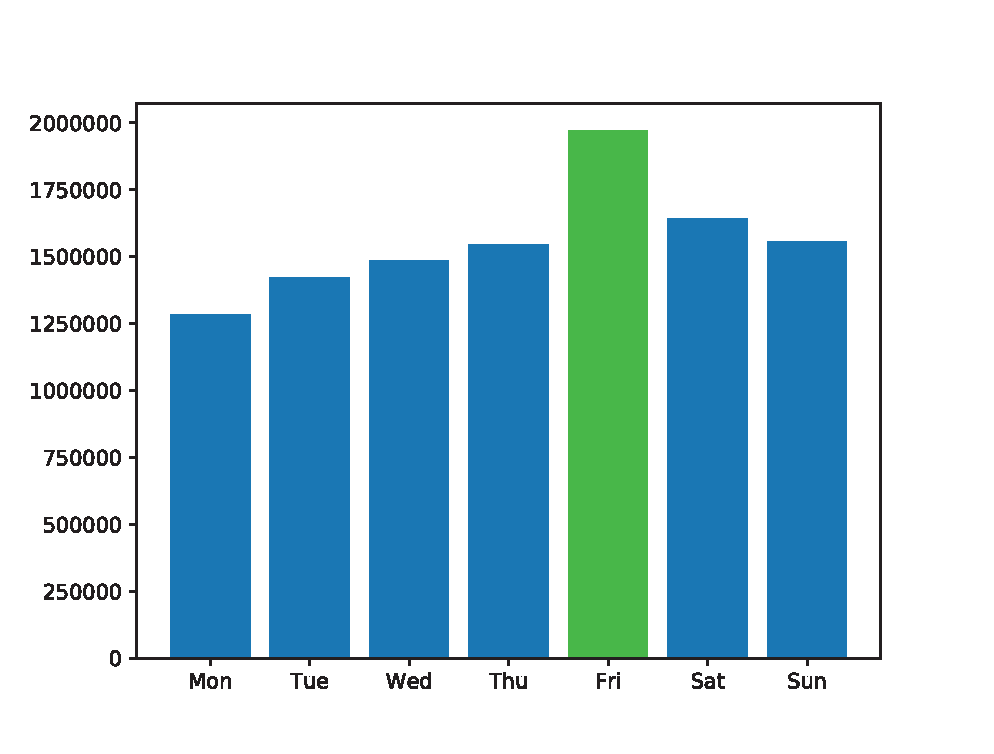
\includegraphics[width=0.5\columnwidth]{observationexample}
  \end{center}

  \caption{An histogram showing an example observation}
  \label{fig:observation_example}
\end{figure}
Observations are features in the data that the user wants to explain. Observations are defined as arithmetic expressions over a set of aggregate queries. Let $F$ be the fact table in our star schema dataset. In the course of this document, we will be using relational algebra expressions defined by \cite{elmasri2011fundamentals} for aggregate expressions. Thus, the $\mathscr{F}$ symbol represents an aggregate function. An aggregate query is defined as:
$$_A\mathscr{F}_B(D), A \in F$$
$B$ is an aggregate function. Examples of an aggregate function include SUM, COUNT, and AVERAGE.
We use SQL to construct an example for an observation. Queries~\ref{qry:aggregateexample1} and \ref{qry:aggregateexample2} show examples of aggregate queries.

Observations made on data can also be represented on histograms. Fig.~\ref{fig:observation_example} shows an example of an observation. The green bar on the histogram represents an aggregate query where the day is Friday.

\renewcommand{\lstlistingname}{Query}% Listing -> Algorithm
\begin{lstlisting}[language=SQL, caption=Aggregate Query for average tip percentage with credit cards, label=qry:aggregateexample1]
SELECT AVG(trip_percentage) FROM
FROM nyc_data
WHERE payment_type = 1
\end{lstlisting}

\renewcommand{\lstlistingname}{Query}% Listing -> Algorithm
\begin{lstlisting}[language=SQL, caption=Aggregate Query for average tip percentage with cash, label=qry:aggregateexample2]
SELECT AVG(trip_percentage) FROM
FROM nyc_data
WHERE payment_type = 2
\end{lstlisting}

Using these aggregate queries we may form an observation based on the ratio of tip percentage with credit card against tip percentage with cash.
$$observation = \frac{\textnormal{Query.~\ref{qry:aggregateexample1}}}{\textnormal{Query.~\ref{qry:aggregateexample2}}}$$


\section{Explanations}
We represent explanations as a predicate. A predicate is a conditional statement which results in a boolean value. We go into more details for the formal definition of different kinds of explanations in Section~\ref{sec:taxonomy}. If we consider Queries~\ref{qry:aggregateexample1} and \ref{qry:aggregateexample2} as an example. The explanation would be in the form of a predicate:
$$tip\_percentage = 15.3$$

Let $D$ be our solution space. We can define our predicate to be the function $P$. Our explanation can now be formally defined as:

\begin{equation}
x|P(x):=
    \begin{cases}
      \text{true}, & \text{if}\ x \in D \\
      \text{false}, & \text{otherwise}
    \end{cases}
\end{equation}

Note that $P$ is an open ended function. In the case of spatial explanations, it can take the form of a spatial function like $ST_CONTAINS$ i.e. whether a polygon contains a point.

\section{K-Folds Cross Validation}
K Folds cross validation is a technique for data evaluation\citep{kohavi1995study,refaeilzadeh2009cross}. The data is divided into $k$ parts. One of the parts is used as a training set and the remaining parts are used as test sets. The purpose of the training set is to model the data. Once we have a model, we can use it to classify and/or predict the unseen data. The test set is used to evaluate how well the model was trained.

\section{Precision and Recall}
Precision and Recall are methods for evaluation\citep{olson2008advanced,powers2011evaluation}. Whenever we classify data we may have true positives, false positive, true negative and false negatives. Precision is defined as:
$$precision = \frac{\textnormal{true positives}}{\textnormal{false positives} + \textnormal{true positives}}$$

Recall is defined as:
$$recall = \frac{\textnormal{true positives}}{\textnormal{true positives} + \textnormal{false negatives}}$$

\section{Distributed Processing Frameworks}
Map Reduce\citep{dean2008mapreduce} is a framework for data processing which is designed for taking distributed and parallel computation into perspective. There are three main operations in a mapreduce process: map, shuffle and reduce. The map operation assigns a key to each element and performs any necessary transformations. The shuffle operation relocates the elements such that elements with the same key are nearby(since they are going to need each other in calculations). The reduce step performs a calculation on each element with the same key and returns the output.

Spark\citep{shanahan2015large,zaharia2016apache} is a distributed and parallel processing framework. The Spark uses a directed acyclic graph to perform calculations. Since the DAG created by Spark can have a lot of common nodes between tasks, the computational complexity of the operation is reduced compared to MapReduce.

Geospark~\citep{yu2015geospark} is a framework for performing several spatial operations on data in Apache Spark. It also has a component which helps in data visualizations\citep{yu2018src}.

\section{Front End Visualization Tools}
React\citep{reactjs} is a front end framework which originated in Facebook. React framework allows interfaces to be designed using Components. Each component has properties and a state. A component can have subcomponents. This makes it simpler to design interfaces which show consistent data across components. Some of the charts included in the interface make use of the eCharts library\citep{echarts}.

MapBox\citep{mapbox} is a library for displaying maps. The maps provided by mapbox consists of tiles and vectors. Each tile represents a cube of the map while vectors are shapes which represent roads, buildings etc. Deck.gl\citep{deckgl} is a library for creating an overlay on top of the map. Examples of overlays include scatterplots, cartograms etc. Matplotlib was also used for static plots for evaluation\citep{hunter2007matplotlib}.
